\section{Actividad No 02 – Reconociendo la estructura} 

\begin{enumerate}[1.]
	\item Crear la tabla Departamentos utilizando la siguiente estructura:
	\\
           \\create table Departamentos (
		\\ID int not null,
		\\nombre varchar (25))
		\\go
	\begin{center}
	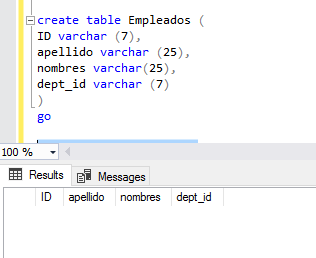
\includegraphics[width=10cm]{./Imagenes/prac2eje1} 
	\end{center}
	\item Poblar la tabla Departamentos con los datos de la tabla Departments.
	\\
		\\create table Empleados (
		\\ID varchar (7),
		\\apellido varchar (25),
		\\nombres varchar(25),
		\\dept\_id varchar (7))
		\\go
	\begin{center}
	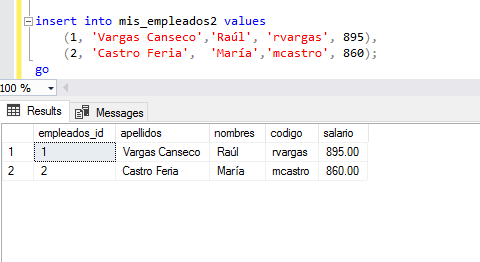
\includegraphics[width=10cm]{./Imagenes/prac2eje2} 
	\end{center}
	\item Crear la tabla Empleados utilizando la siguiente estructura.
	\\
	\\create table mis\_empleados2(
	\\empleados\_id	int not null,
	\\apellidos		varchar(25),
	\\nombres			varchar(25),
	\\codigo			varchar(10),
	\\salario			decimal(9,2))
	\\go
	\begin{center}
	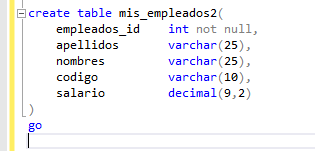
\includegraphics[width=10cm]{./Imagenes/prac2eje3} 
	\end{center}
	\item Crear la tabla Empleados2 basada en la estructura de la tabla Employees. Incluir solo las columnas EMPLOYEE\_ID, FIRST\_NAME, LAST\_NAME, SALARY y DEPARMENT\_ID 		respectivamente.
	\\
	\\create table mis\_empleados3(
	\\empleados\_id	int not null,
	\\apellidos		varchar(25),
	\\nombres			varchar(25),
	\\codigo			varchar(10),
	\\salario			decimal(9,2))
	\\go
	\begin{center}
	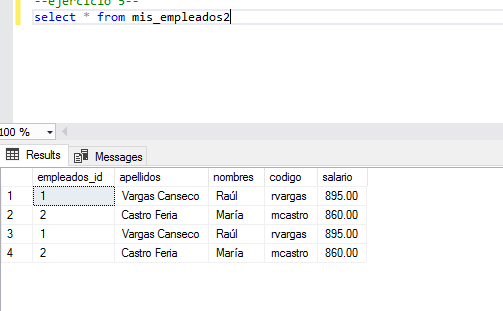
\includegraphics[width=10cm]{./Imagenes/prac2eje5} 
	\end{center}
	\item Modificar el estado de la tabla Empleados2 a SOLO LECTURA.
	\item Tratar de adicionar el siguiente registro a la tabla Empleados2.
	\\
	\\insert into mis\_empleados2 values
	\\(1, 'Vargas Canseco','Ra\'ul', 'rvargas', 895),
	\\(2, 'Castro Feria',  'Mar\'ia','mcastro', 860);
	\\go
	\item Revertir el estado de la tabla LECTURA / ESCRITURA. Tratar de insertar nuevamente la información del punto 4.6.
	\item Eliminar la tabla Empleados2.
	\\
	\\drop table mis\_empleados2
	\begin{center}
	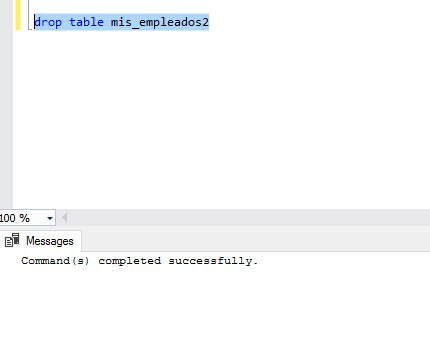
\includegraphics[width=10cm]{./Imagenes/prac2eje8} 
	\end{center}
	
\end{enumerate}